\chapter{PROPOSED SOLUTION}
\label{chap:solution}

This chapter describes a proposed solution which is a considerable system consists of two subsystems: Crowd-sourcing system and  analysis system. In \textit{System overview} subsection, system is briefly described altogether. In two last subsections, structure and details of two subsystems are defined comprehensively.

\section{System overview}
\subsection{Requirement analysis}
To be able to utilize data to serve a security purpose, the most obvious method would be to analyze visual data such as photos and videos.  In recent years, advancements in Artificial Intelligence, especially in Neural Networks, significantly enhanced the development of computer vision field. Project Adam from Microsoft() The use of Deep learning comes along with needs for proper datasets. There are really few datasets that are suitable for the environment of Vietnam. 
The traditional way to collect data would be to set up an array of cameras, then
Crowd-sourcing is one of the effective methods of data collection. The idea behind crowd-sourcing is to build datasets with the help of a large group of people. An example of this kind of model is Wikipedia. Wikipedia is an enormous web-based, collaborative encyclopedia which has over 100,000 volunteers contributing new information to the system daily. The success of Wikipedia proves that people gladly contribute to a system without profit if it brings a greater good. 
But how can people be encouraged to contribute their knowledge and information? Through interaction with others had been proven successful in increasing engagement. Social media has been a popular trend among Vietnamese people. Therefore, this thesis proposes building a social media platform for security. This social media serves as a point of interaction with users, as well as allow people to contribute their knowledge to the system.
Figure \ref{chap3:system_overview_basic} shows an concise overview of how the system operate. Users interact with the \textbf{Crowd-sourcing system} through \textbf{User Interfaces}. Input of users can come in the form of images, videos or label contribution. Inputs of users are stored in the database. The system also be responsible for obtaining appropriate contents from database to display to users through user interfaces.
\begin{center}
    \begin{figure}[H]
    \centering
    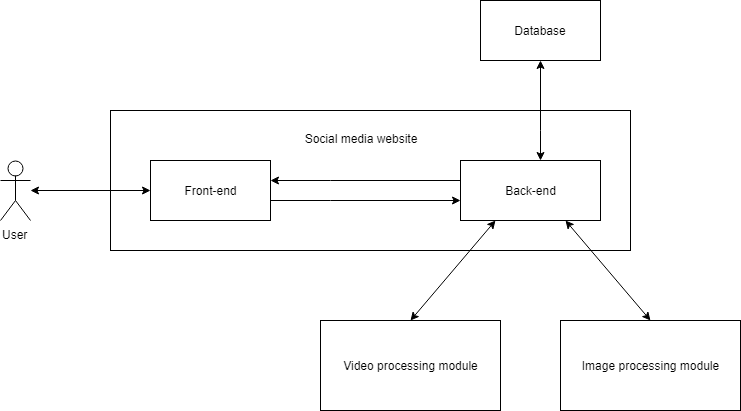
\includegraphics[width=1\columnwidth]{images/chap3/system_overview_basic.png}
    \footcaption{An overview of the system}
    \label{chap3:system_overview_basic}
    \end{figure}
\end{center}
Whenever there is a video to analyze,the server will send it to the \textbf{Video classifier module}, then get the results back. Results returned from video classifier module are classified activity from the video and frames that contain faces in them. \textbf{Face Recognition module} does the job of identifying people in images. Results of both \textbf{Video classifier module} and \textbf{Face Recognition module} are used to determine security threats each video or image shows.
\section{Crowd-sourcing system}
\subsection{Database}
The project database divides into two different parts: \textbf{Cloud storage} and a \textbf{NoSQL database}. Why it requires such a complex system? The primary target is to reduce website loading time. Let take an example, if files are stored directly on the crowd-sourcing server. When many users request a file simultaneously, the server with limited bandwidth will cause delay. “53\% of mobile site visitors leave a page that takes longer than three seconds to load” – \href{https://think.storage.googleapis.com/docs/mobile-page-speed-new-industry-benchmarks.pdf}{Google}. What if these files stored on cloud storage? The client will be served by the cloud storage provider, which has higher availability.
\section{Analysis system}
The project requires two systems for analysis: A face recognition system and a video classifier system. The facial recognition system takes pictures of human faces as input and return their identification. The video classifier system analyzes videos to find out actions in them. The remaining of this section describes in detail about the two analysis system.
\subsection{Face recognition module}
\subsection{Video classifier module}
